% !TeX program = XeLaTeX
% !TeX encoding = UTF-8
% nikachu2012 default TeX template v1.4
% Compiler : XeLaTeX
% TeX ver  : TeX Live 2023
\documentclass[a4paper, xelatex, ja=standard, 10.5pt]{bxjsarticle}
\setpagelayout*{top=25truemm,bottom=25truemm,left=25truemm,right=25truemm}
\addtolength{\headsep}{\topskip}
\setlength{\headsep}{15pt}
\setlength{\footskip}{30pt}

% パッケージインストール
\usepackage{plisting}
\usepackage{docmute}

% 文書開始
\begin{document}

% 概要
% \begin{abstract}
% 概要入力欄。不要な場合は削除してください。
% \end{abstract}

% \maketitle
% \tableofcontents
% \thispagestyle{empty}
% \clearpage

\section{問題設定}
\begin{lstlisting}
Hello.
私は小野です。
\end{lstlisting}
という2行のメッセージを画面に表示する.

\section{問題分析}
今回の問題はターミナル上に英語と日本語のメッセージを表示させれば良い.
まず「\tt{Hello.}」と半角英語で表示して改行し,
次に「\tt{私は小野です。}」と全角日本語で表示して改行する.
そしてプログラムを終了させれば良い.

本プログラム作成にあたり,
標準入出力(stdard input output)ヘッダファイルの\tt{<stdio.h>},
文字列を表示する\tt{printf()},
改行の制御文字\tt{\textbackslash n}を用いる.

\section{設計}
以下に今回作成するプログラムのフローチャートを示す.

\begin{figure}[H]
\centering
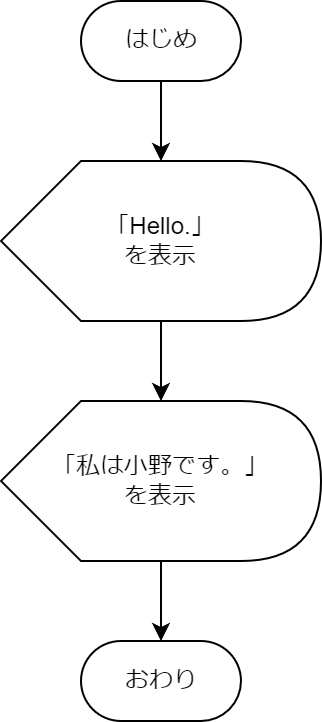
\includegraphics[scale=0.5]{img/flowchart.drawio.png}
\caption{フローチャート}
\label{}
\end{figure}

\section{実装}
まず今回書いたコードを載せる.
\begin{lstlisting}[caption=ソースコード,label=]
/*************************************************
例題1 メッセージの表示[ex01.c]
**************************************************/

#include <stdio.h> // standard input output ヘッダを読み込む

int main(void) // main関数のはじまり
{
    printf("Hello.\n");         // "Hello."を表示
    printf("私は小野です。\n"); //"私は小野です。"を表示
    return 0;                   // 0を返し正常終了したことを伝える
}
\end{lstlisting}
各行で行っていることについてはその都度コメントで記載してあるが,
補足しておく必要があるものもあるので追加で説明する.

まず\tt{\#include <stdio.h>}で「standard input output ヘッダを読み込む」と書いてある.
C言語には関数についてまとめたファイルを読み込む機能があり,
そのうちよく使われるもの(今回で言えば\tt{printf()})などは標準ライブラリと呼ばれるものに入っており,
そのうちの一つとして標準入出力のファイルを読み込んでいる.

ターミナルからの結果は以下の通りである.
\begin{figure}[H]
\centering
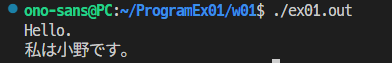
\includegraphics[scale=1.0]{img/wsl_result.png}
\caption{実行結果}
\label{}
\end{figure}
なお適当につけた名前のためふざけているが気にしないでほしい.
一応GitHubでは同じ名前を使っているがその他SNSでは使っていないので
詮索しようと思っても無駄である.

\section{検証}
\section{考察}
\section{タイピング速度測定}
\section{所感}

% 参考文献
\begin{thebibliography}{9} % 数字の最大の桁数分9追加
  \bibitem{key1}example 工学基礎I\hspace{-1.2pt}I\hspace{-1.2pt}I
\end{thebibliography}
\end{document}